\documentclass[11pt,a4paper]{article}
\usepackage[T1]{fontenc}
\usepackage[margin=2.3cm]{geometry}
\usepackage{amsmath,amssymb}
\usepackage{graphicx}
\usepackage[dvipsnames]{xcolor}
\usepackage{enumitem}
\usepackage[colorlinks=true,linkcolor=blue,urlcolor=blue]{hyperref}
\setlength{\parskip}{0.6em}
\setlength{\parindent}{0pt}
\begin{document}

\begin{center}{\LARGE\bfseries openemwave}\\[0.4em]{\large Watch an antenna radiate: electric and magnetic fields, in three sessions.}\\[0.2em]\small PAN IIT OSS explainer \textbullet{} secondary school to diploma / undergraduate (levels 3-5)\end{center}

\section*{Why this exists}
An antenna turns an electrical signal into a travelling wave of electric and magnetic fields. This explainer builds that picture from charges and field lines, through wavelength and antenna length, to a small simulator that marches the fields forward in time.

\section*{The end goal}
Watch an antenna radiate and visualise electric and magnetic fields. The end goal is to watch an antenna radiate and to visualise its electric and magnetic fields: the same tools are used to design phone, wifi and radar antennas, from a single dipole to arrays that steer a beam electronically.

\section*{How the three sessions build up}
\begin{enumerate}[nosep]
\item \textbf{Session 1: Charges, fields and waves} (Level 1, conceptual interactive model, 60 min).
\item \textbf{Session 2: The numbers: Coulomb, superposition and the wave equation} (Level 2, mathematical engineering model, 75 min).
\item \textbf{Session 3: A wave simulator you can trust: FDTD} (Level 3, simulation and validation, 90 min).
\end{enumerate}

\section{Session 1: Charges, fields and waves}

\subsection*{A. Real-world problem}
A balloon rubbed on hair sticks to the wall, and the same kind of invisible push carries your favourite FM station through walls to a small radio. What is that push, how can we draw it, and why are radio waves and light really the same thing? Without this picture, an antenna is just a mysterious piece of metal.

\subsection*{B. Concept and theory}
Electric charge comes in two signs. Charges of the same sign repel and charges of opposite sign attract. The electric field at a point is the push per unit charge that a tiny positive test charge would feel there; it points away from positive charges and towards negative ones, and it is the sum (as arrows) of the pushes from every charge. Two equal positive charges give zero field exactly halfway between them; a dipole (equal positive and negative charges) gives its strongest field there, pointing from the positive towards the negative charge. A wave is a disturbance that moves without carrying the material along: a bump that was at x = 0 at time 0 is at x = v t after time t. For a repeating wave, the wavelength lambda is the distance between crests and the frequency f is the number of crests passing each second, so the wave advances f lambda metres per second: v = f lambda. Radio, wifi, infrared, visible light and X-rays are all electromagnetic waves: they have the same speed in vacuum, c about 3 x 10\textasciicircum{}8 m/s, and differ only in frequency.

\begin{itemize}[nosep]
\item q: electric charge (signed) (coulomb, C (nC = 1e-9 C))
\item E: electric field (push per unit charge) (volt per metre, V/m)
\item v: wave speed (metre per second, m/s)
\item f: frequency (hertz, Hz (1 MHz = 1e6 Hz))
\item lambda: wavelength (metre, m)
\item c: speed of light in vacuum (299 792 458 m/s, about 3e8 m/s)
\end{itemize}

\begin{equation*}
\mathbf E=\sum_i q_i\,\frac{\mathbf r-\mathbf r_i}{|\mathbf r-\mathbf r_i|^{3}}\quad\text{(simple units: sum of the pushes)}
\end{equation*}

\begin{equation*}
y(x,t)=y_0(x-vt)\quad\text{(a bump moving right at speed } v)
\end{equation*}

\begin{equation*}
v=f\,\lambda
\end{equation*}

\begin{equation*}
\lambda=\frac{c}{f},\qquad c\approx 3\times10^{8}\ \mathrm{m/s}
\end{equation*}

\begin{center}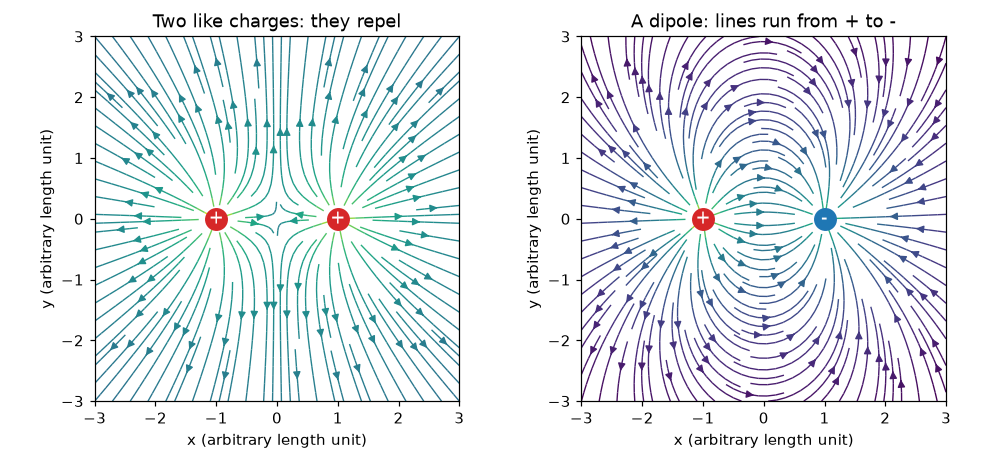
\includegraphics[width=0.85\linewidth]{figures/s01_field_lines.png}\\\small Field lines of two like charges (left) and of a dipole (right).\end{center}

\subsection*{E. Worked example}
An FM station broadcasts at 100 MHz. What is the wavelength of its radio wave? What is the wavelength of 2.4 GHz wifi? Which is longer, and by how much?
\begin{enumerate}[nosep]
\item Use lambda = c / f with c = 2.998 x 10\textasciicircum{}8 m/s.
\item FM: f = 100 MHz = 1.00 x 10\textasciicircum{}8 Hz, so lambda = 2.998e8 / 1.00e8 = 2.998 m, about 3.0 m.
\item Wifi: f = 2.4 GHz = 2.4 x 10\textasciicircum{}9 Hz, so lambda = 2.998e8 / 2.4e9 = 0.1249 m, about 12.5 cm.
\item The ratio of the wavelengths is 2.998 / 0.1249 = 24, which is just the ratio of the frequencies, 2400 / 100 = 24.
\item Sanity check: a human-sized wave (metres) for FM, a hand-sized wave (centimetres) for wifi: this is why FM antennas are long and wifi antennas are short.
\end{enumerate}
\textbf{Answer.} FM: about 3.0 m. Wifi: about 12.5 cm. The FM wave is 24 times longer because its frequency is 24 times lower.

\subsection*{F. Questions}
\begin{enumerate}[nosep]
\item \textbf{Conceptual.} Two protons and two electrons are placed in a line. Explain, without calculating, which pairs push apart and which pull together. Why does the field of two equal positive charges vanish halfway between them?
\item \textbf{Numerical.} A radio wave has frequency 90 MHz. Find its wavelength. Check that the answer is sensible by comparing with the 100 MHz result.
\item \textbf{Graph and simulation interpretation.} In the lambda-versus-frequency graph, FM radio, wifi and green light lie on one straight line. What does that tell you about their speeds? If you moved a point above the line, what would it mean?
\item \textbf{Design and optimisation challenge.} Design: you want a wave whose wavelength is 1 m so that it fits a room-sized test. What frequency do you need? Is that a radio or a light wave? Would a 1 m wave pass through a 5 cm gap in a wall as easily as a 12.5 cm wifi wave?
\end{enumerate}

\section{Session 2: The numbers: Coulomb, superposition and the wave equation}

\subsection*{A. Real-world problem}
How long must the antenna of an FM radio be, and why is the antenna inside a wifi router only a few centimetres long? The answer is a number, and it comes from the speed of light, the frequency and one rule about how antennas work. Along the way we need to put real numbers on the electric field of charges and write the shape of a wave as one equation.

\subsection*{B. Concept and theory}
Coulomb's law gives the size of the electric field of a point charge q at distance r: E = K \textbar{}q\textbar{} / r\textasciicircum{}2 with the Coulomb constant K about 8.99 x 10\textasciicircum{}9 N m\textasciicircum{}2 / C\textasciicircum{}2. The field points away from a positive charge. Fields add as vectors (superposition), so the field of any set of charges is the sum of the fields of each one; a dipole (+q and -q a distance d apart) has, far along its axis, the field 2 K q d / r\textasciicircum{}3 which falls faster than a single charge because the two pushes nearly cancel. A travelling wave is written y(x, t) = A sin(k x - w t): A is the amplitude, k = 2 pi / lambda the wavenumber (radians per metre) and w = 2 pi f the angular frequency (radians per second). A crest keeps k x - w t constant, so it moves at v = w / k = f lambda, which is c for light and radio. A half-wave dipole antenna is a straight conductor of length L = lambda / 2: the wave pushes the electrons back and forth along it in step with the wave. The direction of the wave's electric field is its polarisation; an antenna (or a polarising filter) tilted by theta from that direction receives a fraction cos\textasciicircum{}2(theta) of the power.

\begin{itemize}[nosep]
\item K: Coulomb constant (8.99e9) (N m\textasciicircum{}2 / C\textasciicircum{}2)
\item q: charge (C)
\item r: distance (m)
\item d: separation of the two dipole charges (m)
\item A: wave amplitude (same unit as y)
\item k: wavenumber 2 pi / lambda (rad/m)
\item w: angular frequency 2 pi f (rad/s)
\item L: antenna length (m)
\item theta: angle between receiver and the electric field direction (degrees)
\end{itemize}

\begin{equation*}
E=\frac{K\,|q|}{r^{2}},\qquad K\approx 8.99\times10^{9}\ \mathrm{N\,m^{2}/C^{2}}
\end{equation*}

\begin{equation*}
\mathbf E_{\mathrm{total}}=\sum_i \mathbf E_i\quad\text{(superposition)},\qquad E_{\mathrm{dipole}}\approx \frac{2Kqd}{r^{3}}\ \ (r\gg d)
\end{equation*}

\begin{equation*}
y(x,t)=A\sin(kx-\omega t),\qquad k=\frac{2\pi}{\lambda},\ \ \omega=2\pi f,\ \ v=\frac{\omega}{k}=f\lambda
\end{equation*}

\begin{equation*}
L=\frac{\lambda}{2}=\frac{c}{2f},\qquad \frac{P_{\mathrm{received}}}{P_{\max}}=\cos^{2}\theta
\end{equation*}

\begin{center}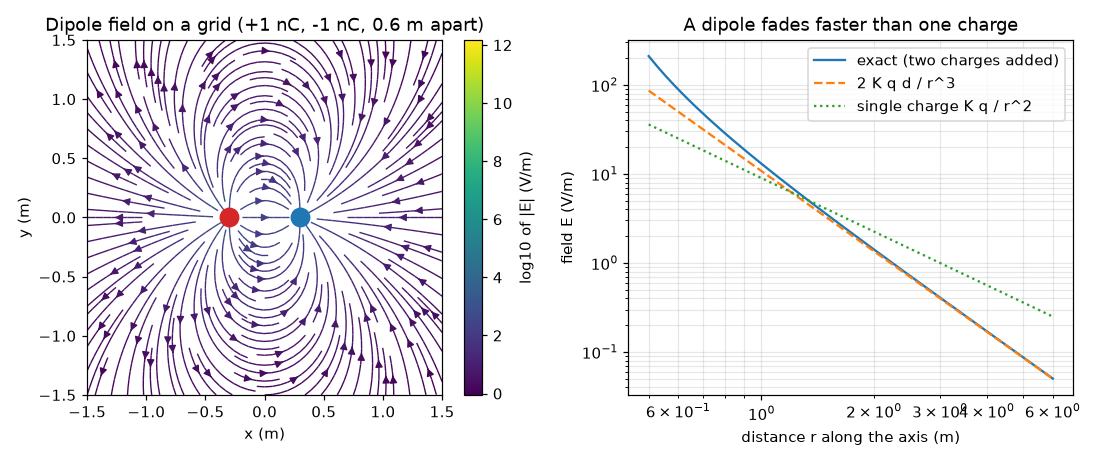
\includegraphics[width=0.85\linewidth]{figures/s02_dipole_field.png}\\\small A dipole computed on a grid, and its field on the axis against distance.\end{center}

\subsection*{E. Worked example}
A 2.4 GHz wifi wave: find lambda, k, w and check that w / k = c. Then find the half-wave antenna length. Finally compute the field of a 1 nC charge at 0.5 m.
\begin{enumerate}[nosep]
\item lambda = c / f = 2.998e8 / 2.4e9 = 0.1249 m = 12.5 cm.
\item k = 2 pi / lambda = 6.283 / 0.1249 = 50.3 rad/m.
\item w = 2 pi f = 6.283 x 2.4e9 = 1.508e10 rad/s.
\item Check: w / k = 1.508e10 / 50.3 = 3.00e8 m/s, which is c.
\item Half-wave antenna: L = lambda / 2 = 0.0625 m = 6.2 cm.
\item Coulomb: E = K q / r\textasciicircum{}2 = 8.99e9 x 1e-9 / 0.5\textasciicircum{}2 = 8.99 / 0.25 = 35.96 V/m, about 36 V/m.
\end{enumerate}
\textbf{Answer.} lambda = 12.5 cm, k = 50.3 rad/m, w = 1.508e10 rad/s, v = w / k = c, antenna 6.2 cm; and 36 V/m for 1 nC at 0.5 m.

\subsection*{F. Questions}
\begin{enumerate}[nosep]
\item \textbf{Conceptual.} Why does the field of a dipole fall off as 1/r\textasciicircum{}3 while the field of a single charge falls off as 1/r\textasciicircum{}2? What would happen if the two charges had the same sign?
\item \textbf{Numerical.} A 2 nC charge. Find the field 0.3 m away. Then find the field if the distance is doubled, and sanity-check the ratio.
\item \textbf{Graph and simulation interpretation.} In the log-log graph of dipole field against distance, the curves for the exact dipole and for 2 K q d / r\textasciicircum{}3 touch at large r but separate at small r. Where do they separate and why? Which line is steeper, the dipole or the single charge?
\item \textbf{Design and optimisation challenge.} Design: choose the length of a half-wave dipole for an FM station at 100 MHz. A rod can be bought only in whole centimetres and your radio case is 1.2 m long. What length do you choose, and what trade-off does a shorter rod cause?
\end{enumerate}

\section{Session 3: A wave simulator you can trust: FDTD}

\subsection*{A. Real-world problem}
Engineers cannot solve Maxwell's equations by hand for a phone antenna or a router in a room, so they simulate the fields on a computer grid and march them forward in time. But a simulation can look beautiful and still be wrong. How do you know that a simulator tells the truth, and when is it lying? Today you build one and test it against five things you already know from theory.

\subsection*{B. Concept and theory}
Maxwell's equations say that a changing magnetic field makes an electric field and a changing electric field makes a magnetic field. In the TMz picture of 2D (electric field Ez out of the page, magnetic field Hx, Hy in the page) and in normalised units with c = 1, eps = mu = 1, the equations become: dHx/dt = -dEz/dy, dHy/dt = dEz/dx, dEz/dt = dHy/dx - dHx/dy. The FDTD method (finite-difference time-domain) puts Ez on whole grid points and Hx, Hy half a cell away (the Yee grid) and updates E and H alternately in half-steps (leapfrog). With the Courant number S = c dt / dx, each update adds S times a difference of neighbouring values. The scheme is stable only if S \textless{}= 1 in 1D and S \textless{}= 1/sqrt(2) in 2D (dt \textless{}= dx / (c sqrt 2)); above that, tiny errors grow every step and the field blows up. Even when stable, a grid slows short waves: the numerical phase speed obeys sin(w dt / 2) = S sin(k dx / 2), which is about 1 - (k dx)\textasciicircum{}2 (1 - S\textasciicircum{}2) / 24 of c, so waves with fewer than about 10 points per wavelength travel noticeably too slowly (numerical dispersion). The grid edge needs an absorbing condition (here the simple first-order Mur rule) or the wave would echo back; a perfect conductor wall (Ez = 0) reflects the wave and makes a standing wave with nodes lambda / 2 apart. A line source in 2D radiates a cylindrical wave whose amplitude falls as 1/sqrt(r) (its power spreads over a circle of length 2 pi r), while a 3D point source falls as 1/r. Two sources a distance d apart with phase difference delta give a far-field amplitude \textbar{}cos((k d cos(theta) + delta) / 2)\textbar{}; the beam points where k d cos(theta) + delta = 0, so changing delta steers it.

\begin{itemize}[nosep]
\item Ez, Hx, Hy: field components in the simulation (normalised units (E and H have the same scale because Z0 = 1))
\item dx: grid cell size (one cell (unit of length))
\item dt, S: time step; Courant number c dt / dx (dt in cell-crossing times; S has no unit)
\item ppw: points (cells) per wavelength (no unit)
\item lambda, k: wavelength in cells; wavenumber 2 pi / lambda (cells; rad/cell)
\item d, delta: source spacing; phase of the second source (cells (or lambda); radians)
\item theta: angle from the line joining the sources (degrees or radians)
\end{itemize}

\begin{equation*}
\frac{\partial H_x}{\partial t}=-\frac{\partial E_z}{\partial y},\quad \frac{\partial H_y}{\partial t}=\frac{\partial E_z}{\partial x},\quad \frac{\partial E_z}{\partial t}=\frac{\partial H_y}{\partial x}-\frac{\partial H_x}{\partial y}
\end{equation*}

\begin{equation*}
E_z^{n+1}=E_z^{n}+S\left[(H_y)_{i}-(H_y)_{i-1}-(H_x)_{j}+(H_x)_{j-1}\right],\qquad S=\frac{c\,\Delta t}{\Delta x}
\end{equation*}

\begin{equation*}
\Delta t\le \frac{\Delta x}{c\sqrt{2}}\ \text{(2D)},\qquad \sin\frac{\omega\Delta t}{2}=S\sin\frac{k\Delta x}{2}
\end{equation*}

\begin{equation*}
|E_z|\propto \frac{1}{\sqrt r}\ \text{(2D wave)},\qquad \text{node spacing}=\frac{\lambda}{2},\qquad |E|\propto\left|\cos\frac{kd\cos\theta+\delta}{2}\right|
\end{equation*}

\begin{center}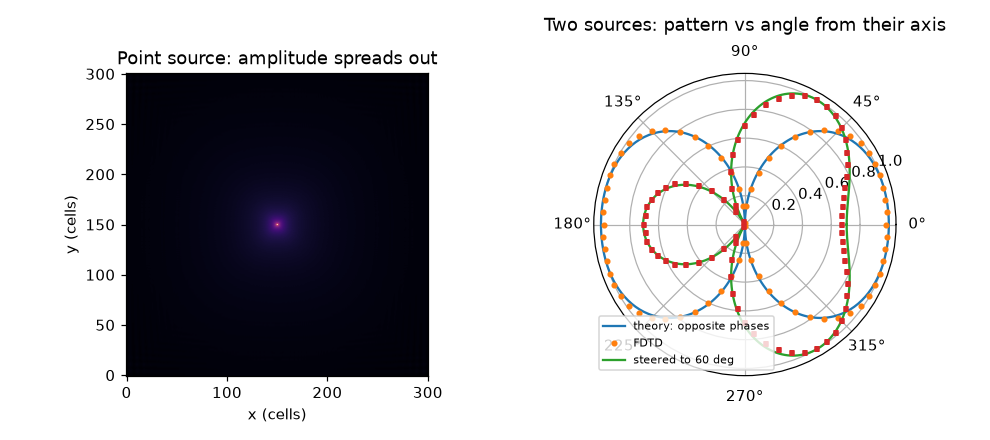
\includegraphics[width=0.85\linewidth]{figures/s03_pattern.png}\\\small Amplitude map of a point source, and the polar pattern of two sources: theory against simulation.\end{center}

\subsection*{E. Worked example}
You want to simulate a 2.4 GHz wifi wave in a 1 m square room with 20 cells per wavelength. Find the cell size, the largest stable time step in 2D, the number of steps per wave period and the number of cells across the room.
\begin{enumerate}[nosep]
\item Wavelength: lambda = c / f = 2.998e8 / 2.4e9 = 0.1249 m.
\item Cell size: dx = lambda / 20 = 0.1249 / 20 = 6.25 mm.
\item Cells across 1 m: 1 / 0.006246 = 160 cells.
\item Courant limit in 2D: dt \textless{}= dx / (c sqrt 2) = 6.246e-3 / (2.998e8 x 1.4142) = 14.73 ps.
\item Period T = 1 / 2.4e9 = 416.7 ps, so the number of steps per period is 416.7 / 14.73 = 28.3 at the limit (more steps are needed if S is smaller than the limit).
\end{enumerate}
\textbf{Answer.} dx = 6.25 mm, 160 cells across, dt at most 14.73 ps, about 28 steps per period at the limit.

\subsection*{F. Questions}
\begin{enumerate}[nosep]
\item \textbf{Conceptual.} Why does a time step above the Courant limit make the simulation blow up, even though the true wave equation is perfectly well behaved? What does S mean physically?
\item \textbf{Numerical.} A grid has 8 points per wavelength and S = 0.5. Estimate the numerical phase speed as a fraction of c using 1 - (k dx)\textasciicircum{}2 (1 - S\textasciicircum{}2) / 24, and say whether the grid is good enough for a 1 percent accuracy.
\item \textbf{Graph and simulation interpretation.} In the point-source amplitude measurement, the fitted slope on a log-log graph is -0.499. What does a slope of -0.5 mean, and what slope would a 3D source give? What would a slope of -1 in the 2D simulation tell you?
\item \textbf{Design and optimisation challenge.} Design: choose the phase difference between two sources a half wavelength apart so that the main beam points 45 degrees from their line, and say whether a spacing of 0.8 lambda is a good idea. Use the hand calculation, then say what you would check in the simulation.
\end{enumerate}

\section{Real-world mini-project}
\textbf{Steer a beam with two sources.} A small-cell radio needs its beam to point 45 degrees away from the line joining its two antennas. The two sources are half a wavelength apart (5 cells at 10 points per wavelength). Use \texttt{ring\_pattern} and \texttt{beam\_phase} from Session 3: the hand calculation tells you roughly what phase difference to use, the simulation tells you what you really get.

\section{The path ahead}
\begin{enumerate}[nosep]
\item \textbf{Session 4: An 8-element steerable array.} A function that drives N sources with a progressive phase and measures the beam in the simulation.
\item \textbf{Session 5: A better absorbing boundary.} A matched absorbing layer around the grid.
\item \textbf{Session 6: A dielectric slab.} A grid with a permittivity map and a slab of refractive index 2.
\item \textbf{Session 7: Go 3D: a point source.} A 3D FDTD solver with a small radiating source.
\item \textbf{Session 8: Animate and share the beam.} A looping GIF of a steered beam.
\end{enumerate}

\section{Answers and hints}

\subsection*{Session 1}
\begin{enumerate}[nosep]
\item \textbf{Conceptual.} Hint: Same sign repels, opposite sign attracts. At the midpoint each charge pushes with the same strength. Solution: Proton-proton and electron-electron pairs have the same sign and repel; proton-electron pairs have opposite signs and attract. Halfway between two equal positive charges each pushes the test charge away from itself, with equal strength but in opposite directions, so the two pushes cancel and the field is zero there.
\item \textbf{Numerical.} Hint: lambda = c / f with c = 3e8 m/s (or 2.998e8). Convert MHz to Hz first. Solution: f = 90 MHz = 9.0e7 Hz, so lambda = 2.998e8 / 9.0e7 = 3.33 m. Sanity check: a lower frequency than 100 MHz must give a longer wavelength than 3.0 m, and 3.33 m is longer. Unit: metres.
\item \textbf{Graph and simulation interpretation.} Hint: On a log-log graph lambda = c / f is a straight line with slope -1; the position of the line is set by c. Solution: They all lie on the same line because lambda f = c is the same for each, so all travel at the same speed c. A point above the line would be a wave with a longer wavelength at the same frequency, so lambda f \textgreater{} c: a wave faster than light in vacuum, which does not happen. (Waves in glass or water are slower than c and would lie below the line.)
\item \textbf{Design and optimisation challenge.} Hint: f = c / lambda. Compare the gap with the wavelength: waves are blocked or bent when the opening is smaller than about a wavelength. Solution: f = 2.998e8 / 1 = 3.0e8 Hz = 300 MHz, a radio wave (between FM and wifi). A 5 cm gap is much smaller than 1 m and also smaller than 12.5 cm, so neither passes easily as a straight beam; the 12.5 cm wave is closer to the gap size and passes much better. Assumptions: simple picture of a gap; the real behaviour depends on the material and on how the wave is shaped.
\end{enumerate}

\subsection*{Session 2}
\begin{enumerate}[nosep]
\item \textbf{Conceptual.} Hint: At a large distance the two fields point almost the same way but have opposite signs for a dipole. Solution: For a dipole the two charges are almost the same distance away, so their fields are almost equal and opposite and nearly cancel; only the small difference caused by the separation d remains, which is why the result is smaller and falls faster (2 K q d / r\textasciicircum{}3). With the same sign the fields would add instead of cancel and the far field would look like a single charge of size 2q, falling as 1/r\textasciicircum{}2.
\item \textbf{Numerical.} Hint: E = K q / r\textasciicircum{}2 with q = 2e-9 C. Solution: E(0.3) = 8.99e9 x 2e-9 / 0.09 = 17.98 / 0.09 = 199.8 V/m, about 200 V/m. At 0.6 m: 17.98 / 0.36 = 49.9 V/m. The ratio 199.8 / 49.9 = 4, as expected for an inverse square law (double the distance, a quarter of the field).
\item \textbf{Graph and simulation interpretation.} Hint: The formula assumes r is much bigger than d. Solution: They separate at small r, close to the charges (at r = 0.5 m with d = 0.6 m the formula is not valid because r is not much larger than d), and agree for large r. The dipole line is steeper (slope -3) than the single-charge line (slope -2).
\item \textbf{Design and optimisation challenge.} Hint: L = c / (2 f); then compare with what fits. Solution: L = 2.998e8 / (2 x 1e8) = 1.499 m, about 1.5 m, which does not fit in a 1.2 m case. Options: fold or telescope it, or use a shorter antenna (for example a quarter-wave, 0.75 m, over a conducting plane). A shorter rod than lambda / 2 still receives, but it is a poorer match to the wave, so the received signal is weaker. Assumption: ideal thin rod; a real one is cut a few percent shorter.
\end{enumerate}

\subsection*{Session 3}
\begin{enumerate}[nosep]
\item \textbf{Conceptual.} Hint: S = c dt / dx is the fraction of a cell the wave crosses in one step. Solution: S is the fraction of a cell the wave travels in one time step. If S is too large the numerical scheme asks a cell to depend on information that physically has not yet reached it; the rounding error that is always present is then amplified every step instead of damped, and it grows exponentially. The true equation does not have this problem, so the blow-up is a property of the discretisation. In 2D the limit is 1/sqrt(2) because the wave can also travel along the diagonal of a cell.
\item \textbf{Numerical.} Hint: k dx = 2 pi / ppw. Solution: k dx = 2 pi / 8 = 0.785. (k dx)\textasciicircum{}2 = 0.617. (1 - S\textasciicircum{}2) = 0.75. So the error is 0.617 x 0.75 / 24 = 0.0193 and the phase speed is about 0.981 c, 1.9 percent slow. That is worse than 1 percent, so 8 points per wavelength is not enough; at 10 points per wavelength the error is 1.2 percent and at 12 about 0.9 percent.
\item \textbf{Graph and simulation interpretation.} Hint: Amplitude \textasciitilde{} r\textasciicircum{}p, so the slope of log(amplitude) against log(r) is p. Solution: A slope of -0.5 means amplitude falls as 1/sqrt(r): as r grows 4 times, amplitude halves; power (amplitude squared) falls as 1/r, because it spreads over a circle of length 2 pi r. A 3D point source spreads over a sphere of area 4 pi r\textasciicircum{}2, so power falls as 1/r\textasciicircum{}2 and amplitude as 1/r: slope -1. A slope of -1 in the 2D run would signal that energy is being lost (for example a very absorbing medium) or a mistake in the measurement, such as measuring too close to the source or after the wave hit a boundary.
\item \textbf{Design and optimisation challenge.} Hint: cos(theta0) = -delta / (k d). Compare k d with 2 pi. Solution: k d = 2 pi x 0.5 = pi, cos 45 = 0.707, so delta = -pi x 0.707 = -2.22 rad = -127 degrees (a phase step of -130 degrees in the simulation gives about 44 degrees). A spacing of 0.8 lambda is a poor idea: with k d = 1.6 pi a second solution of k d cos(theta) + delta = 2 pi appears, a grating lobe, so a second unwanted beam appears. In the simulation check that the measured peak on the ring is within a few degrees of 45 and that there is no second lobe of similar size. Trade-off: a wider spacing gives a narrower beam but risks grating lobes.
\end{enumerate}

\section{How to join}
Read \texttt{CONTRIBUTING.md} in the repository, then pick an issue labelled \texttt{good first issue}. Repository: \url{https://github.com/KrunalPanchal1995/openemwave}

\end{document}
